\section{Durchführung}
\begin{figure}
    \centering
    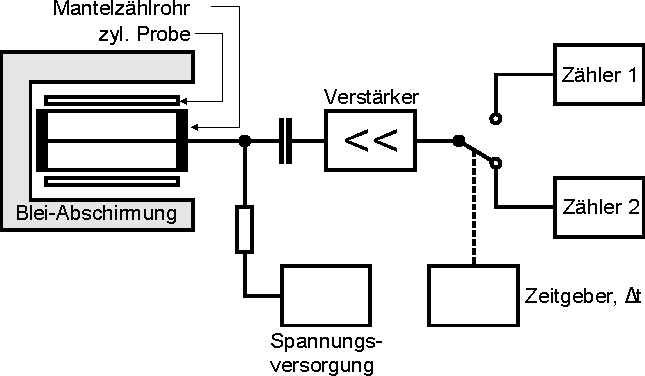
\includegraphics{Abbildungen/Schaltplan.pdf}
    \caption{Aufbau der Messanlage \cite{man:v702}}
    \label{fig:Aufbau}
\end{figure}
Die Messungen erfolgen mit der In Abb. \ref{fig:Aufbau} skizzierten Apparatur.
Mit einem Geiger-Müller-Zählrohr werden die von den Proben emittierten
$\beta$- und $\gamma$-Teilchen gemessen. 
Der Verstärker macht es möglich die gemessenen Teilchen 
in den Zählmaschinen zu zählen. 
In einer Angemessenen Zeit $\Delta t$ wird das Signal zwischen den
Zählmaschinen hin und her geschaltet.
Das Messgerät wird durch eine Bleiwand von der äusseren 
Hintergrundstrahlung abgeschirmt. 
Trotzdem existiert ein sogenannter Nulleffekt, Strahlung 
die ohne hinzufügen von einer Radioaktiven Strahlungsquelle gemessen werden kann.
Dieser Nulleffekt wird in der ersten Messreihe gemessen. 
Anschliessend wird die Strahlung der in \ref{fig:neutronenquelle}